\ifpdf
    \graphicspath{{figures/}{figures/comparisons}}
\else
    \graphicspath{{figures/}{figures/comparisons}}
\fi

%: ----------------------- name of chapter  -------------------------
\chapter{Implementation} % top level followed by section, subsection
This chapter describes the chosen implementation environment. It also describes an Android application which was created in order to acquire image sequences with additional sensor data. The structure of both Android and Desktop projects is explained and essential implementation details of the proposed algorithms and strategies are discussed herein.
\section{Choosing Environment}
Currently, Android has one of the best APIs which allows programmers to acquire sensor fusioned data of rotation and linear acceleration.
In order to avoid coding anew all epipolar geometry algorithms, C++ version of OpenCV library was used. Image acquiring process was seperated from model reconstruction. This allowed to save a lot of time in debugging which is highly difficult in native C++ development on Android. In order to enrich images with sensor data an Android app was created and a standalone C++ desktop app to perform processing and evaluation.
\section{Project Structure} \label{sec:ProjectStructure}
Source codes of both applications can be found on an attached CD and in the Github repository at the following web address: TODO \url{https://github.com/KrzysztofWrobel/MasterThesisSource.git}. In general, the project was split into two subprojects: Android and Desktop. In addition, some of the sample datasets were added to the dataset folder in order to perform evaluations similar to the ones described in the next chapter.
\section{"Sensor Enhanced Images Camera" - Android Gradle based project}
In order to capture images and associate them with sensor data, a custom photo capture app called "Sensor Enhanced Images Camera" was created.
Using this application, the camera orientation angles can be tracked in real-time in reference to the Earth's coordinate system. Also linear acceleration, current velocity and relative translation from the location of the last picture taken can be tracked. 
Upon the photo capture the current camera rotation and relative translation are stored in a custom JSON file. A corresponding image is saved along with this JSON file in folder, which is created upon every app start-up. It allows for taking different dataset captures without them being mixed up.
\subsection{Installation}
In order to compile and distribute Android application, a Gradle based built system was used. This is currently a recommended way to maintain Android based projects [TODO ref. google]. At present this app supports only devices with Android 4.0 and above. In order to compile this project it is recomended to install Android Studio, which already contains the needed SDK and also has a built-in Gradle support. More information about configuration, compilation and installation steps can be found in README.md in the main catalog of the attached source code. 
\subsection{User Interface}
As mentioned earlier the app allows to track all necessery external camera parameters in real-time. This is how the first version of user interface looked:
\begin{figure}[h!]
    \centering
    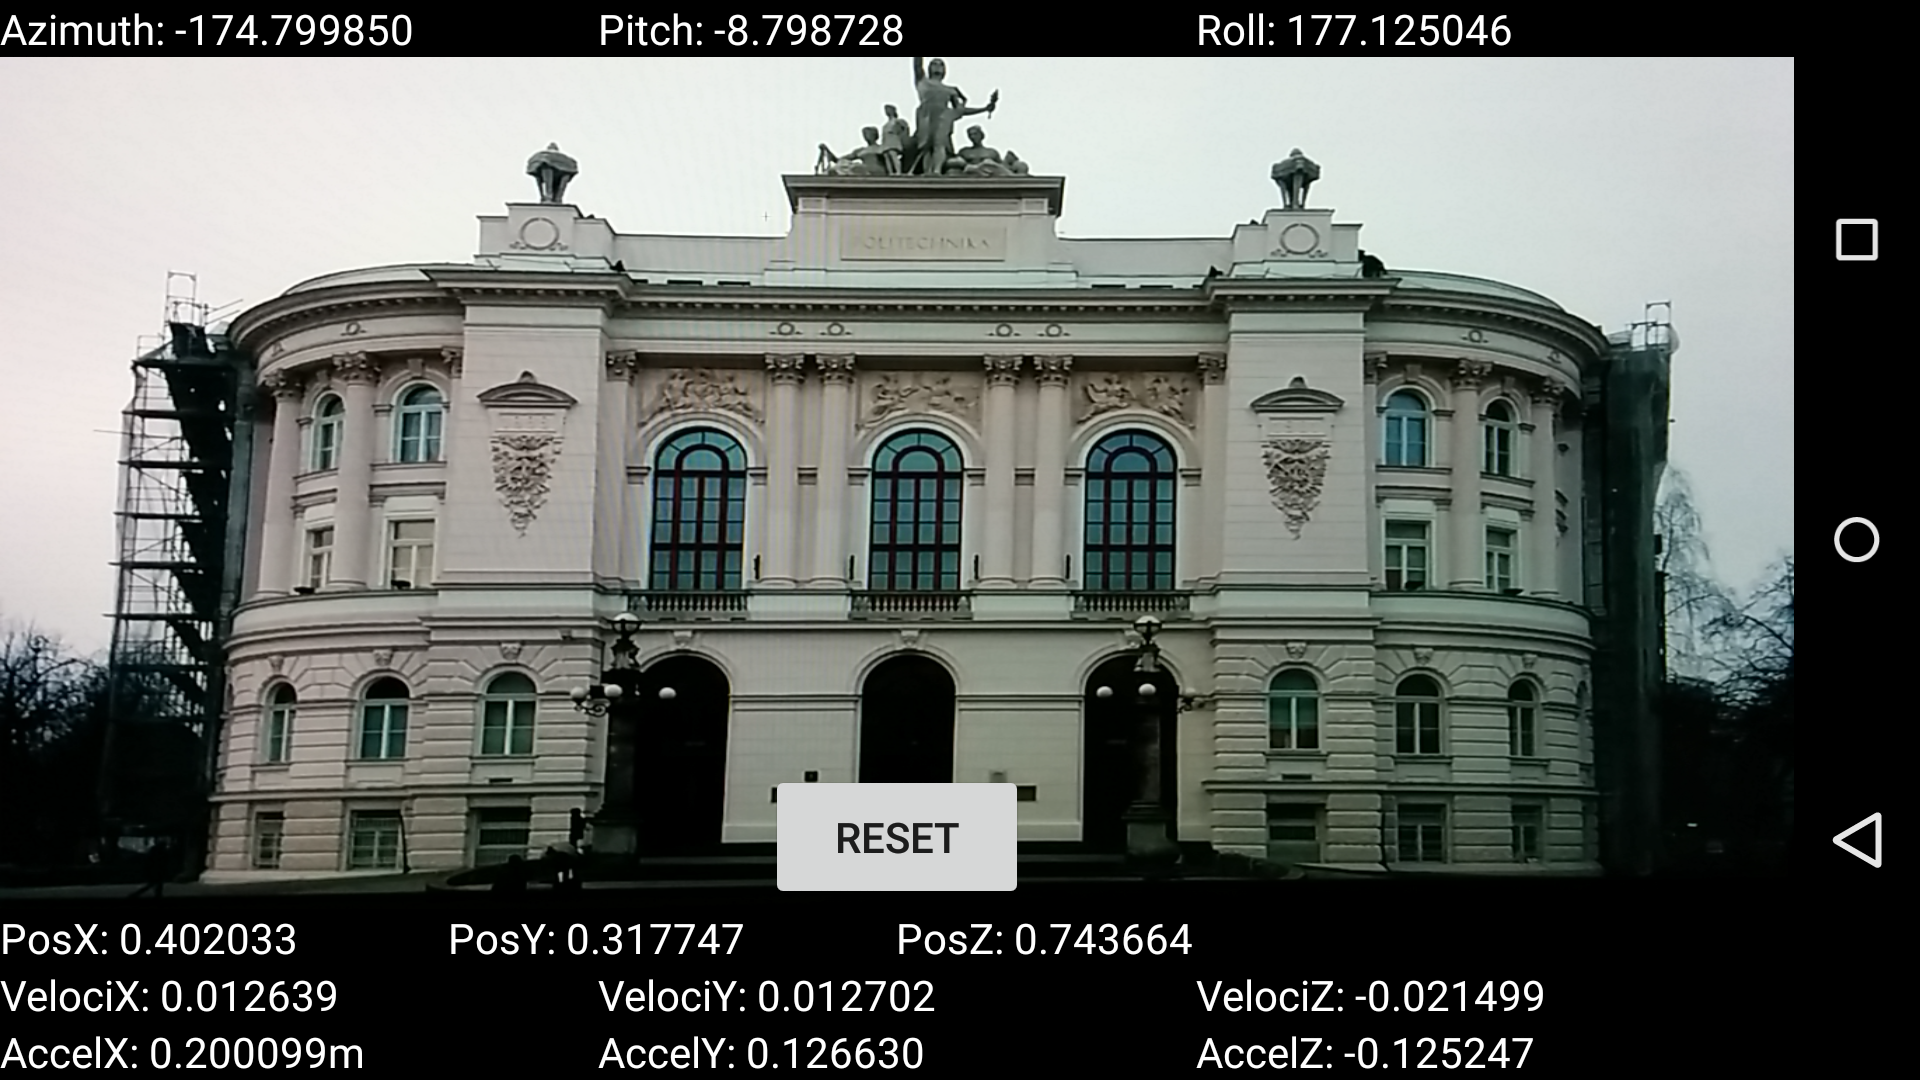
\includegraphics[width=0.8\textwidth]{AndroidScreenShot}
    \caption{}
    \label{fig:AndroidScreenShot}
\end{figure}
\clearpage
In order to capture a photo, a user only has to click on the screen center. No additional configuration is required. To use the so acquired datasets in another program, the smartphone has to be connected to the computer. Folders are created with time suffixes in the main catalog of an internal SD card.
\subsection{Important Implementation Aspects}
There were two important aspects of an Andoid application implementation:
\begin{enumerate}
\item Camera rotation calculation
\item Heuristcal movement estimation
\end{enumerate}
\subsubsection{Rotation calculation}
Android SDK already has a built-in API, which can be used to access sensor fusioned data. In particular, for measuring the rotation, the $Sensor.TYPE\_ROTATION\_VECTOR$ was used. It returns 9-degree quaternion in reference to geomagnetic north pole. In order to decompose it to euler angles a helper method was used:
\lstset{escapechar=@,style=customjava}
\begin{lstlisting}
private float[] euclidanAnglesFromQuaternion(float[] quaternion) {
        ...
        //Converts quaternion to 4x4 rotation matrix
        SensorManager.getRotationMatrixFromVector(rotMat, quaternion);
        ...
        //Extracts euclidan Angles in radians
        SensorManager.getOrientation(rotMat, orientation);
        ...
        return orientation;
}
\end{lstlisting}
\subsubsection{Custom heuristics for move estimation}
Using the currently available Android sensor data it is difficult to estimate the relative translation of the device. Linear accelaration measurments, which can be accessed with $Sensor.TYPE\_LINEAR\_ACCELERATION$ constant, are very noisy. Such noisy data with double intergration over time results in quite big errors after some time. First integration is required to acquire current velocity change. Second integration over velocity is required to calculate position change in particular moment.
However, it can be improved using human-walking model description with the following heuristical constraints over calculated velocity:
\begin{enumerate}
\item When new linear acceleration sensor data is ready, first apply lowPass filtering in order to reduce some high frequency noise.
\item Change sensor datda vector from local camera coordinates to global reference system (multiply with inverted rotation matrix)
\item Decide depending on current state, if deviceMovmentState has changed:
\begin{enumerate}
\item If device was previously IDLE and incoming Acceleration value is bigger than $0.5\frac{m}{s^2}$ change device state to MOVING and reset current velocity to $0\frac{m}{s}$
\item If device was previously MOVING and incoming Acceleration value is smaller than $0.1\frac{m}{s^2}$ change device state to IDLE
\end{enumerate}
\item Only if device is currently moving:
\begin{enumerate}
\item Update device velocity
\item Check current speed with walk constraint (People walk with avarage speed of $1.5\frac{m}{s}$) and eventually scale it down to maximum value
\item Update device postion
\end{enumerate}
\end{enumerate}
A code snippet of the described movement estimation heuristics was derived from Android application and can be found in the following listing \ref{lst:positionHeuristic}. Maximum walking speed can be adjusted, but by default it should be set to around $1.5\frac{m}{s}$ TODO \url{http://en.wikipedia.org/wiki/Preferred_walking_speed}. 
The most important factor of the accurate reconstruction are correletions between movements in X,Y and Z axes. Noise in sensors is equally distributed on each axis, so it estimated translation should keep these movements' correlations properly.

\begin{lstlisting}[caption={Snippet from Android source code position estimation heuristic},label={lst:positionHeuristic},numbers=left,escapeinside={@}{@},float]
    public void onSensorChanged(SensorEvent event) {
            ...
        } else if (event.sensor == mLinearAcceleration) { 
            ...   
            //Filtering out some noise
            newGlobalAcceleration = lowPass(newGlobalAcceleration, currentGlobalAcceleration);
            //Switch linear acceleration from phone local coordinates to global coordinates
            Matrix.multiplyMV(newGlobalAcceleration, 0, invertedRotationMatrix.clone(), 0, newGlobalAcceleration, 0);

            double distance = getLength(currentGlobalAcceleration);
            long currentTimeMillis = System.currentTimeMillis();
            //Decide state of the device. Distance is in m/s^2
            if (distance > 0.5 && deviceState == State.IDLE) {
                if (currentTimeMillis - movingEndTime > 300) {
                    deviceState = State.MOVING;
                    currentGlobalVelocity = {0,0,0};
                }
            } else if (distance < 0.1 && deviceState == State.MOVING) {
                if (currentTimeMillis - movingStartTime > 350) {
                    deviceState = State.IDLE;
                }
            }

            if (deviceState == State.MOVING) {
                //Update current device velocity
                currentGlobalVelocity += currentGlobalAcceleration * dT;
                
                double velocity = getLength(currentGlobalVelocity);
                //Check and adjust current velocity. People walk with avarage speed 1.5\frac{m}{s}
                if (velocity > WALKING_MAX_VELOCITY) {
                    currentGlobalVelocity /= velocity / WALKING_MAX_VELOCITY;
                }
                
                //Update device relative position, s = V0 * t + a * t^2/2;
                currentRelativePosition += currentGlobalVelocity * dT + currentGlobalAcceleration * dT * dT / 2;                 
            }
            ...
    }   
\end{lstlisting}

\subsubsection{Custom Sensor Data File format}
As mentiond earlier each photo sensor information is stored in a separe file. By default the following information is stored for each captured image:
\begin{itemize}
\item \textbf{ID}, which indicates order of the photos
\item \textbf{Path}, which relates the path to a corresponding image file
\item \textbf{Euler Angles - pitch, roll, azimuth}
\item \textbf{Relative position coordinate}
\end{itemize} 
All these pieces of information are stored as a list and when the user has completed taking pictures, entire information set is saved into JSON file named sensor.txt. A sample file can be found in the Additional Materials[TODO].\pagebreak

\section{"Enhanced 3D Reconstructer" - OSX CMake-based project}
In order to evaluate algorithms there was a need to prepare a comfortable project environment which would allow for numerical and visual comparison of multiple datasets. CMake was choosen in order to simplify building and compilation process. The entire code architecture was developed and tested on Apple MacbookAir with OSX 10.9 Mavericks. In order to compile this project the following elements need to be installed first:
\begin{itemize}
\item CMake 2.8
\item OpenCV 2.4.10
\item Point Cloud Library (PCL) 1.7
\item Boost 1.55
\item cvsba \url(http://www.uco.es/investiga/grupos/ava/node/39) [TODO reference move]
\end{itemize}
\subsection{User Interface}
There are two targets defined in CMake file:
\begin{enumerate}
\item \textbf{Test efficiency}, which was used to evaluate pair reconstruction methods, draw epipolar lines in images and calculate samson error distances
\item \textbf{Test reconsturction}, which was used to evaluate proposed initialization pair reconstruction methods with different pose estimation methods
\end{enumerate}
\subsubsection{Test Efficiency}
There is no graphical interface for reconstruction parameters configuration. All parameters needed are configured from the command-line interface. The following parameters have to be configured for this purpose:
\begin{enumerate}
\item \textbf{Enhanced Photo Data folder path}
\item \textbf{Initial SIFT features set size}
\end{enumerate}
The calculated execution times and execution time are printed to the console output.
\subsubsection{Test reconstruction}
There is no graphical interface for reconstruction parameters configuration either. All neccessary parameters have to be configured from the command-line interface. The following variables need to be configured:
\begin{enumerate}
\item \textbf{Enhanced Photo Data folder path}
\item \textbf{Initial SIFT features set size}
\item \textbf{Init pair reconstruct method}
\begin{itemize}
\item Standard 8-point algorithm
\item Enhanced 8-point algorithm
\item Standard 5-point algorithm
\item Enhanced 5-point algorithm
\item Alternative 3-point translation estimation
\item None (use existing rotations and translations informations)
\end{itemize}
\item \textbf{Pose estimation method:}
\begin{itemize}
\item Standard OpenCV Pose Estimation
\item Rotation enhanced Pose Estimation 
\item Rotation and translation enhanced Pose Estimation
\item None (use existing rotations and translations)
\end{itemize}
\item \textbf{Whether drop outliers or not}
\item \textbf{Whether use Bundla Adjustment or not}
\end{enumerate}
The output received by the user is a reconstructed model in a file with *.asc extension. The reconstructed model is also visible in PCL Visualizer integrated into the code. The user can navigate through the model with mouse and 'F' key, which centers the camera view on a selected point.
\subsection{Important Implementation Aspects}
Most of the necessary algorithms were already implemented in OpenCV. In addition an opensource project with 5-point algorithm implementation was used. Its source code can be found here: [TODO reference].
\subsubsection{Rotation matrix generation}
To parse Android generated sensor data file Boost JsonParser was used. As mentioned earlier, Android saves decomposed Euler angles. In order to properly multiply this angles to acquire a proper rotation matrix the following code inspired on MathWorld Wolfram [TODO \url{http://mathworld.wolfram.com/EulerAngles.html}]
\begin{lstlisting}
Mat getRotation3DMatrix(double pitch, double azimuth, double roll) {
    Mat D = (Mat_<T>(3, 3) <<
            cos(roll), -sin(roll), 0,
            sin(roll), cos(roll), 0,
            0, 0, 1);

    Mat C = (Mat_<T>(3, 3) <<
            cos(azimuth), 0, -sin(azimuth),
            0, 1, 0,
            sin(azimuth), 0, cos(azimuth));
    Mat B = (Mat_<T>(3, 3) <<
            1, 0, 0,
            0, cos(pitch), -sin(pitch),
            0, sin(pitch), cos(pitch));
    //Important
    return B * C * D;
}
\end{lstlisting}
\subsubsection{Enhancing epipolar equations}
As could have been observed in \ref{sec:EpipolarEquation}, in order to enhance initial pair reconstruction algorithms same as the standard ones can be used, but with specially conditioned point matching. The standard 8-point algorithm is already available in OpenCV library. The implemented enhanced 8-point version can be found in 'Multiview.cpp' file, but its main difference is that it uses sets of specially modified input points, which are conditioned and the first one is additionaly rotated with Initial Rotation Matrix. In OpenCV it can be done with:
\begin{lstlisting}
    ...
    undistortPoints(points1Exp, points1Exp, K, distCoeffs, rotDiffGlobal);
    undistortPoints(points2Exp, points2Exp, K, distCoeffs);
    ...
\end{lstlisting}
where rotDiffGlobal is the relative rotation matrix between two cameras. The estimated fundamental matrix needs to be transformed to essential matrix for further decomposition. In order to choose proper matrix decomposition the following code is used:
\begin{lstlisting}
void chooseProperMatrixFromEnhanced(Mat &dRx, Mat &dR1x, Mat &TdRExp, Mat &dR, Mat &T) {
    dR = dRx;
    if (decideProperMatrix(dRx, 0.05)) {
        dR = constraintMatrix(dRx);
    } else if (decideProperMatrix(dR1x, 0.05)) {
        dR = constraintMatrix(dR1x);
    } else if (decideProperMatrix(-dRx, 0.05)) {
        dR = constraintMatrix(-dRx);
    } else if (decideProperMatrix(-dR1x, 0.05)) {
        dR = constraintMatrix(-dR1x);
    }

    Mat skewT = TdRExp * dR.inv();
    cout << "skewT" << skewT << endl;

    Mat tdecx = Mat(3,1, CV_64FC1);
    tdecx.at<double>(0) = (skewT.at<double>(2,1) - skewT.at<double>(1,2))/2;
    tdecx.at<double>(1) = (skewT.at<double>(0,2) - skewT.at<double>(2,0))/2;
    tdecx.at<double>(2) = (skewT.at<double>(1,0) - skewT.at<double>(0,1))/2;
    T = tdecx;

}

bool decideProperMatrix(Mat dRot, double tolerance){
    double a00 = abs(dRot.at<double>(0,0) - 1);
    double a11 = abs(dRot.at<double>(1,1) - 1);
    double a22 = abs(dRot.at<double>(2,2) - 1);
    if((a00 + a11 + a22)/3< tolerance) {
        return true;
    }else {
        return false;
    }
}
\end{lstlisting}
These lines help to decide on a properly constrained rotation error matrix \ref{eq:rodiguesError} and calculate relative translation between cameras.
\subsubsection{Alternative 3-point translation estimation}
When it is known or assumed that the acquired rotation data is accurate, the translation can be calculated with the 3-point algorithm. The ones proposed in \ref{eq:alternative3point} and \ref{eq:translation3point} were implemented. Similarily to other epipolar estimations methods implemented in OpenCV, this one also has the ability to properly filter outliers with the use of RANSAC algorithm is used. The following listing contains this implementation:
\begin{lstlisting}
    ...
    for (iterationNumber = 0; iterationNumber < niters; iterationNumber++) {

        getSubsety(prev_points_raw, next_points_raw, point1s, point2s, 300, modelPoints);
        Mat t = findTranslation(point1s, point2s, rotDiffGlobal, Kinv);
        Mat F1 = constructFundamentalMatrix(rotDiffGlobal, t, Kinv);

        int goodCount = findInliersy(prev_points_raw, next_points_raw, F1, errors, statuses, reprojThreshold);
        if (goodCount > maxGoodCount) {
            swap(statuses, goodStatuses);
            FEnhanced = F1;
            tEnhanced = t / t.at<double>(2);
            maxGoodCount = goodCount;
            niters = cvRANSACUpdateNumIters(confidence,
                    (double) (count - maxGoodCount) / count, modelPoints, niters);
        }

    }
    ...
    
    
    Mat findTranslation(std::vector<cv::Point2d> &points1, std::vector<cv::Point2d> &points2, Mat &rotDiff, Mat &Kinv) {

    Mat hg1 = Mat::zeros(points1.size(), 3, CV_64FC1);
    Mat hg2 = Mat::zeros(points2.size(), 3, CV_64FC1);
    for (int i = 0; i < points1.size(); i++) {
        hg1.at<double>(i, 0) = points1[i].x;
        hg1.at<double>(i, 1) = points1[i].y;
        hg1.at<double>(i, 2) = 1;
        hg2.at<double>(i, 0) = points2[i].x;
        hg2.at<double>(i, 1) = points2[i].y;
        hg2.at<double>(i, 2) = 1;
    }

    hg1 = hg1 * (rotDiff * Kinv).t();
    hg2 = hg2 * (Kinv).t();

    Mat A = Mat::zeros(hg1.rows, 3, CV_64FC1);
    for (int i = 0; i < hg1.rows; i++) {
        A.at<double>(i, 0) = (hg2.at<double>(i, 2) * hg1.at<double>(i, 1) - hg2.at<double>(i, 1) * hg1.at<double>(i, 2));
        A.at<double>(i, 1) = (hg2.at<double>(i, 0) * hg1.at<double>(i, 2) - hg2.at<double>(i, 2) * hg1.at<double>(i, 0));
        A.at<double>(i, 2) = (hg2.at<double>(i, 1) * hg1.at<double>(i, 0) - hg2.at<double>(i, 0) * hg1.at<double>(i, 1));
    }

    SVD svd1(A);
    Mat tCalc = svd1.vt.row(2);

    //Translation between cameras estimated and Fundamental Matrix from that as well
    Mat T = (tCalc.t());

    return T;

\end{lstlisting}
\subsubsection{Enhancing pose estimation}
OpenCV already has the rotation and translation enhanced pose estimation implemented. The only thing that has to be done is performing the conversion of euclidan rotation matrix to its Rodrigues representation. The initial rotation and translation need to be passed as input variables. Pose estimation methods implementations are as follows: 
\begin{lstlisting}
Mutiview::FindPoseEstimation(
        cv::Mat &rvec,
        cv::Mat &t,
        cv::Mat &R,
        cv::Mat &K,
        cv::Mat &distCoeffs,
        std::vector<cv::Point3d> ppcloud,
        std::vector<cv::Point2d> imgPoints,
        vector<int> inliers) 
Mutiview::FindPoseEstimationEnhanced(
        cv::Mat &rvec,
        cv::Mat &t,
        cv::Mat &R,
        cv::Mat &RInit,
        cv::Mat &TInit,
        cv::Mat &K,
        cv::Mat &distCoeffs,
        std::vector<cv::Point3d> ppcloud,
        std::vector<cv::Point2d> imgPoints,
        vector<int> inliers)
\end{lstlisting}
can be found in 'Mutiview.cpp' file.


% ---------------------------------------------------------------------------
%: ----------------------- end of thesis sub-document ------------------------
% ---------------------------------------------------------------------------

